\section{Opis implementacije i prikaz praktičnog dijela rada}

\subsection{Instalacija i početno postavljanje}

Instalacija nove Next.js aplikacije jednostavna je i započinje izvršavanjem
naredbe \texttt{npx create-next-app@latest} u terminalu uz željeni naziv
projekta kao argument. Nakon pokretanja slijede interaktivne upute u terminalu,
dok se pri korištenju zastavice \texttt{-{}-yes} projekt automatski
inicijalizira s predefiniranim postavkama (omogućen TypeScript, Tailwind CSS,
ESLint, App Router, Turbopack te alias za uvoz \texttt{@/*})~\cite{nextJsDocs}.
Nakon uspješne instalacije, aplikacija je spremna za pokretanje i razvoj.

Naredba \texttt{next dev} pokreće razvojni poslužitelj i koristi Turbopack kao
zadani \textit{bundler}, što omogućuje vrlo brze inkrementalne
\textit{buildove} i osvježavanje promjena tijekom razvoja. \texttt{next build}
priprema aplikaciju za produkciju optimiziranjem k\^oda, generiranjem statičkih
stranica i pakiranjem resursa, dok \texttt{next start} pokreće produkcijski
poslužitelj nad prethodno izgrađenom verzijom aplikacije. Skripta
\texttt{eslint} služi za pokretanje alata ESLint, koji automatski provjerava
stil i potencijalne pogreške u JavaScript/TypeScript k\^odu.

Dobra je praksa i odmah inicijalizirati Git repozitorij u projektu, što se može
učiniti naredbom \texttt{git init}. To omogućuje praćenje promjena i
upravljanje verzijama k\^oda tijekom razvoja.

Također, preporučeno je postaviti i formatiranje k\^oda, što se može postići
instalacijom i konfiguracijom alata poput Prettiera kako bi se osigurao
dosljedan stil k\^oda. EditorConfig datoteka također može pomoći u održavanju
dosljednosti postavki između različitih uređivača k\^oda i razvojnih okruženja.

\subsection{Struktura Next.js projekta}

\subsubsection{Struktura početnog direktorija}

Osnovna struktura \textit{root} direktorija implementirane Next.js aplikacije
jest sljedeća:\\ \dirtree{.1 repeticije-hr/. .2 {.next/}. .2 app/. .2
  calendar/. .2 components/. .2 data/. .2 lib/. .2 middleware/. .2
  node\_modules/. .2 prisma/. .2 public/. .2 scripts/. .2 services/. .2
  supabase/. .2 {.editorconfig}. .2 {.env}. .2 {.env.example}. .2 {.gitignore}.
  .2 {.prettierrc.json}. .2 components.json. .2 eslint.config.mjs. .2
  next-env.d.ts. .2 next.config.ts. .2 package-lock.json. .2 package.json. .2
  postcss.config.mjs. .2 prisma.config.ts. .2 proxy.ts. .2 README.md. .2
  tsconfig.json. .2 vercel.json. }%

\begin{itemize}
  \item \texttt{.next/} {--} Automatski generiran direktorij koji sadrži rezultat procesa izgradnje (kompajlirane stranice, \textit{bundleove} i \textit{cache}) te se ne verzionira u sustavu za kontrolu verzija.
  \item \texttt{app/} {--}  Sadrži rute, \textit{layoute} i API rute temeljene na Next.js App Routeru, odnosno predstavlja glavni k\^od korisničkog sučelja i poslužiteljske logike unutar okvira Next.js.
  \item \texttt{calendar/} {--}  Izdvojeni paket s komponentama, kontekstima i pomoćnim funkcijama za rad s kalendarom (preuzet s \texttt{\href{https://github.com/lramos33/big-calendar}{github.com/lramos33/big-calendar}}) i prilagođen za potrebe aplikacije.
  \item \texttt{components/} {--}  Sadrži višekratno iskoristive React komponente korisničkog sučelja, od osnovnih UI elemenata do složenijih komponenti.
  \item \texttt{data/} {--}  Implementira sloj pristupa podatcima (engl.\ \textit{repository layer}) nad bazom podataka, s modulima za korisnike, ponude repeticija, rezervacije itd.
  \item \texttt{lib/} {--}  Zajedničke pomoćne biblioteke i konfiguracije, uključujući autentikaciju, Prisma klijent, Supabase klijent, WebRTC signalizaciju i opće \textit{utility} funkcije.
  \item \texttt{middleware/} {--}  Sadrži middleware k\^od za zaštitu ruta; sadrži implementirane funkcije za provjeru autentikacije i autorizacije nad dolaznim zahtjevima.
  \item \texttt{node\_modules/} {--}  Automatski generiran direktorij s instaliranim \texttt{npm} paketima, tj.\ \textit{runtime} i \textit{build} ovisnostima projekta.
  \item \texttt{prisma/} {--}  Sadrži datoteku \texttt{schema.prisma} s modelom baze podataka, SQL migracije te skriptu \texttt{seed.ts} za inicijalno popunjavanje baze.
  \item \texttt{public/} {--}  Statički resursi (slike, ikone, SVG-ovi i sl.) koji su javno dostupni bez dodatne obrade na poslužiteljskoj strani.
  \item \texttt{scripts/} {--}  Pomoćne skripte za održavanje i pozadinske zadatke (npr.\ \textit{cron} skripta za automatsko ažuriranje statusa rezervacija).
  \item \texttt{services/} {--}  Implementacija poslovne logike aplikacije, koja koristi repozitorije za pristup podatcima i implementira funkcionalnosti specifične za domenu.
  \item \texttt{supabase/} {--}  Konfiguracijske datoteke i dokumentacija za lokalno okruženje Supabase i migracije baze.
  \item \texttt{.editorconfig} {--}  Datoteka s pravilima formatiranja k\^oda za različite uređivače k\^oda.
  \item \texttt{.env}, \texttt{.env.example} {--}  Datoteke s konfiguracijskim varijablama okruženja (stvarna konfiguracija i ogledni primjer).
  \item \texttt{.gitignore} {--}  Definira koje datoteke i direktoriji se isključuju iz verzioniranja.
  \item \texttt{.prettierrc.json} {--}  Konfiguracija za Prettier formatiranje k\^oda.
  \item \texttt{components.json} {--}  Konfiguracijska datoteka za sustav komponenti.
  \item \texttt{eslint.config.mjs} {--}  Konfiguracija ESLint-a za statičku analizu k\^oda.
  \item \texttt{next-env.d.ts} {--}  TypeScript deklaracije specifične za Next.js, automatski generirane.
  \item \texttt{next.config.ts} {--}  Glavna konfiguracijska datoteka Next.js aplikacije (\textit{build} postavke, usmjeravanje, integracije).
  \item \texttt{package-lock.json} {--}  Zaključane verzije \texttt{npm} paketa za determinističke instalacije.
  \item \texttt{package.json} {--}  Metapodatci o projektu te popis \texttt{npm} skripti i ovisnosti.
  \item \texttt{postcss.config.mjs} {--}  Konfiguracija za PostCSS \textit{pipeline} (npr. Tailwind CSS).
  \item \texttt{prisma.config.ts} {--}  Pomoćne postavke i funkcije povezane s Prismom i bazom podataka.
  \item \texttt{proxy.ts} {--}  Implementira \textit{proxy} logiku i zaštitu API ruta; koristi \textit{middleware} funkcije za kontrolu pristupa.
  \item \texttt{README.md} {--}  Osnovna projektna dokumentacija i upute za pokretanje.
  \item \texttt{tsconfig.json} {--}  Konfiguracija TypeScript kompajlera.
  \item \texttt{vercel.json} {--}  Konfiguracija \textit{deploymenta} na platformu Vercel.
\end{itemize}

\subsubsection{Struktura direktorija \texttt{app/}}

Struktura direktorija \texttt{app/} zasebno je predstavljena zbog svoje ključne
uloge u organizaciji k\^oda i implementaciji poslovne logike aplikacije. Unutar
direktorija \texttt{app/} nalaze se sljedeći poddirektoriji i datoteke:\\

\dirtree{.1 app/. .2 (auth)/. .2 (main)/. .2 api/. .2 generated/. .2
  apple-icon.png. .2 favicon.ico. .2 globals.css. .2 icon0.svg. .2 icon1.png. .2
  layout.tsx. .2 manifest.json. }%

\begin{itemize}
  \item \texttt{(auth)/} {--} Grupa ruta koja sadrži stranice vezane uz autentikaciju (prijava, registracija, zaboravljena lozinka, ponovno postavljanje lozinke); ove rute su odvojene od ostatka aplikacije radi jasne organizacije.
  \item \texttt{(main)/} {--} Glavna grupa ruta. Sadrži sve ostale stranice aplikacije koje nisu vezane uz autentikaciju, poput početne stranice, stranica s ponudama repeticija, profilom korisnika, stranica nadzorne ploče itd.
  \item \texttt{api/} {--} Sadrži API \texttt{route} datoteke koje implementiraju REST sučelje za rad s korisnicima, tutorima, ponudama repeticija, rezervacijama, recenzijama, predmetima i sobama.
  \item \texttt{generated/} {--} Direktorij u koji Prisma generira klijentski k\^od (Prisma Client) i povezane tipove, koji se potom koriste u poslužiteljskim dijelovima Next.js aplikacije za pristup bazi podataka.
  \item \texttt{apple-icon.png}, \texttt{favicon.ico}, \texttt{icon0.svg}, \texttt{icon1.png} {--} Ikone aplikacije koje se koriste u preglednicima i pri instalaciji kao progresivna web aplikacija (PWA), npr.\ za prikaz na početnom zaslonu mobilnog uređaja.
  \item \texttt{globals.css} {--} Datoteka s globalnim CSS stilovima koji se učitavaju jednom te vrijede za cijelu aplikaciju.
  \item \texttt{layout.tsx} {--} Korijenski \textit{layout} App Routera koji definira zajedničku strukturu stranica (npr.\ zaglavlje, podnožje i pružatelje konteksta).
  \item \texttt{manifest.json} {--} PWA manifest koji opisuje osnovne metapodatke aplikacije te omogućuje „instaliranje” aplikacije na uređaj.
\end{itemize}

\subsection{Dijagram arhitekture aplikacije}

Na slici~\ref{fig:archDiagram} prikazan je dijagram arhitekture implementirane
aplikacije, koji nastoji ilustrirati ključne komponente i slojeve sustava te
njihove međusobne odnose i komunikaciju.

\begin{figure}[H]
  \includegraphics[width=1\linewidth,clip=]{assets/architecture-diagram.png}
  \centering
  \caption{Dijagram arhitekture aplikacije}\label{fig:archDiagram}
\end{figure}

\subsection{Rad s bazom podataka}

Aplikacija koristi bazu podataka PostgreSQL upravljanu na platformi Supabase
kao centralno spremište svih trajnih podataka o korisnicima, ponudama
repeticija, rezervacijama termina, recenzijama i ostalim entitetima domene. Za
pristup bazi koristi se Prisma ORM, koji se na Supabase Postgres spaja putem
stringa za povezivanje (engl.\ \textit{connection string}) preuzetog iz
Supabase sučelja i definiranog u varijablama okruženja aplikacije. Na taj se
način kombiniraju prednosti Supabasea (upravljani PostgreSQL, sigurnost,
nadzor) i Prisma ORM-a (tipizirani upiti, migracije, generirani klijent), bez
potrebe za održavanjem vlastite baze.

\subsubsection{Postavljanje i postupci nad bazom podataka}

Baza podataka kreirana je kao Supabase projekt, pri čemu Supabase osigurava
PostgreSQL instancu. U Supabase sučelju generirani su stringovi za povezivanje
s bazom, koji su zatim spremljeni u \texttt{.env} datoteku Next.js aplikacije
kao varijable \texttt{DATABASE\_URL} i \texttt{DIRECT\_URL}. Te se varijable
koriste za konfiguraciju Prisma ORM-a pri inicijalizaciji, omogućujući mu da se
poveže na PostgreSQL bazu unutar Supabase okruženja.

Prisma ORM služi kao apstrakcijski sloj između domenskog k\^oda i baze podataka
PostgreSQL.\@ U datoteci \texttt{schema.prisma} definiraju se modeli koji
preslikavaju domenske entitete na tablice u bazi podataka, uključujući tipove
stupaca, primarne i strane ključeve te kardinalitet veza. Na temelju te
definicije Prisma generira tipizirani klijent (\texttt{@prisma/client}) koji se
koristi u repozitorijskom sloju aplikacije (\texttt{data/}) za izvođenje upita
i transakcija nad bazom, dok servisni sloj aplikacije (\texttt{services/})
ovisi o repozitorijima umjesto o izravnim SQL upitima, što omogućuje jasnu
separaciju poslovne logike i pristupa podatcima.

U ispisu~\ref{lst:prismaInstallation} prikazane su naredbe koje su korištene za
instalaciju Prisma ORM-a u projektu.

\begin{lstlisting}[caption={Naredbe za instalaciju Prisma ORM-a}, label={lst:prismaInstallation}]
npm install prisma tsx @types/pg --save-dev
npm install @prisma/client @prisma/adapter-pg dotenv pg
\end{lstlisting}

Nakon instalacije potrebno je inicijalizirati Prismu naredbom: \texttt{npx
  prisma init --db --output ../app/generated/prisma}. Ova naredba kreira osnovnu
strukturu datoteka i direktorija potrebnih za rad s Prismom, uključujući
datoteku \texttt{schema.prisma}.

U ispisu~\ref{lst:prismaSchema} prikazan je primjer definicije modela baze
podataka u datoteci \texttt{schema.prisma}.

\begin{lstlisting}[caption={Primjer definicije modela baze podataka u datoteci \texttt{schema.prisma}}, label={lst:prismaSchema}, style=Prisma]
model TutorSubject {
  tutorId String
  subjectId String
  lessonOffers LessonOffer[]
  subject Subject @relation(fields: [subjectId], references: [id])
  tutor User @relation(fields: [tutorId], references: [id])

  @@id([tutorId, subjectId])
}
\end{lstlisting}

Svaki model odgovara jednoj tablici u bazi podataka, a polja unutar modela
definiraju stupce tablice, njihove tipove i odnose s drugim modelima.

Migracije baze podataka kreirane su pomoću Prisma Migrate te se izvršavaju
naredbom: \texttt{npx prisma migrate dev} nakon definiranja ili izmjene modela
u\\ \texttt{schema.prisma}. Ova naredba generira SQL migracijske datoteke koje
se zatim primjenjuju na bazu podataka, stvarajući potrebne tablice i odnose.

Prisma klijent generira se naredbom: \texttt{npx prisma generate} nakon
definiranja modela, čime se omogućuje korištenje tipiziranog API-ja za pristup
bazi podataka unutar aplikacije.

Punjenje baze podataka inicijalnim testnim podatcima izvršeno je naredbom:
\texttt{npx prisma db seed} koja pokreće skriptu \texttt{prisma/seed.ts} za
umetanje testnih zapisa u bazu.

Za administraciju baze i razvoj u lokalnom okruženju korišten je i pomoćni alat
za naredbeni redak Supabase CLI (engl. \textit{Command Line Interface}), koji
omogućuje upravljanje Supabase projektom i bazom podataka iz terminala. Putem
njega je bilo moguće povezati lokalni projekt s udaljenim Supabase projektom,
povući ili primijeniti promjene nad bazom (\texttt{supabase db pull},
\texttt{supabase db push}) te izraditi sigurnosne kopije i izvoze sheme baze
podataka. Za lokalni razvoj korištene su naredbe \texttt{supabase start} i
\texttt{supabase stop}, kojima se pokreće, odnosno zaustavlja kompletan lokalni
Supabase \textit{stack}, što olakšava reprodukciju produkcijskog okruženja na
razvojnom računalu~\cite{supabaseDocs}.

\subsubsection{Dijagram relacijske baze podataka}

Na slici~\ref{fig:erDiagram} prikazan je ER (engl.\ \textit{Entity
  Relationship}) dijagram relacijske baze podataka u sučelju platforme Supabase,
na kojem se mogu vidjeti tablice u koje su podatci spremani i njihove međusobne
relacije.

Relacijska baza podataka sastoji se od 11 tablica:

\begin{itemize}
  \item \texttt{\_prisma\_migrations} {--} tablica koju koristi Prisma za praćenje izvršenih migracija baze podataka.
  \item \texttt{User} {--} glavna tablica koja pohranjuje osnovne podatke o korisnicima.
  \item \texttt{Session}, \texttt{Account}, \texttt{Verification} {--} tablice koje, uz \texttt{User}, koristi autentikacijska biblioteka Better Auth.
  \item \texttt{Subject} {--} tablica koja pohranjuje informacije o predmetima.
  \item \texttt{TutorSubject} {--} povezna tablica koja modelira mnogostruku vezu između tablica \texttt{User} (tutor) i \texttt{Subject}.
  \item \texttt{TutorAvailability} {--} tablica koja pohranjuje dostupnost tutora za pojedine dane i vremenske intervale.
  \item \texttt{LessonOffer} {--} tablica koja pohranjuje ponude repeticija koje su tutori kreirali.
  \item \texttt{Reservation} {--} tablica koja pohranjuje rezervacije koje su korisnici napravili na ponude repeticija.
  \item \texttt{Review} {--} tablica koja pohranjuje recenzije koje su korisnici ostavili tutorima nakon održanih repeticija.
\end{itemize}

\begin{figure}[H]
  \centering
  \includegraphics[width=1\linewidth,clip=]{assets/db-er-diagram.png}
  \caption{Dijagram relacijske baze podataka}\label{fig:erDiagram}
\end{figure}

\subsection{Repozitoriji u sloju pristupa podatcima}

Aplikacija koristi sloj pristupa podatcima (engl.\ \textit{data access layer})
koji se nalazi u direktoriju \texttt{data/} i implementira repozitorije za
različite domenske entitete. Repozitoriji su odgovorni za izvođenje operacija
nad bazom podataka putem Prisma klijenta. Pojedini repozitoriji implementiraju
funkcije za dohvat, kreiranje, ažuriranje i brisanje zapisa u bazi, a servisni
sloj aplikacije koristi te repozitorije za implementaciju poslovne logike bez
direktne ovisnosti o detaljima pristupa podatcima.

U ispisu~\ref{lst:subjectRepo} prikazan je primjer implementacije repozitorija
za entitet \texttt{Subject}.

\begin{lstlisting}[caption={Primjer implementacije repozitorija za entitet \texttt{Subject}}, label={lst:subjectRepo}]
import prisma from "@/lib/prisma"

export class SubjectRepository {
  static async findAll() {
    return prisma.subject.findMany({
      orderBy: { createdAt: "desc" },
    })
  }

  static async findById(id: string) {
    return prisma.subject.findUnique({
      where: { id },
    })
  }

  static async create(name: string) {
    return prisma.subject.create({
      data: { name },
    })
  }

  static async update(id: string, name: string) {
    return prisma.subject.update({
      where: { id },
      data: { name },
    })
  }

  static async delete(id: string) {
    return prisma.subject.delete({
      where: { id },
    })
  }
}
\end{lstlisting}

\subsection{Poslovna logika u servisnom sloju}

Poslovna logika aplikacije implementirana je u servisnom sloju, koji se nalazi
u direktoriju \texttt{services/}. Servisi koriste repozitorije za pristup
podatcima i implementiraju funkcionalnosti koje su specifične za poslovne
procese aplikacije, poput kreiranja ponuda repeticija, rezervacija termina,
ostavljanja recenzija i sl. Servisi su dizajnirani tako da budu neovisni o
specifičnim detaljima baze podataka, što omogućuje fleksibilnost u slučaju
promjena u sloju pristupa podatcima ili migracije na drugi sustav za pohranu.

U ispisu~\ref{lst:lessonOfferService} prikazan je primjer implementacije
servisne funkcije za kreiranje ponude repeticija.

\begin{lstlisting}[caption={Primjer implementacije servisne funkcije za kreiranje ponude repeticija}, label={lst:lessonOfferService}]
import { LessonOfferRepository, TutorRepository } from "@/data"
import { ApiError } from "@/lib/utils/error-handler"
import { LessonMode, LessonType, LocationMode } from "@/app/generated/prisma/enums"

export class LessonOfferService {
  static async createLessonOffer(data: {
    tutorId: string
    subjectId: string
    durationMin: number
    type: LessonType
    capacity: number
    price: number
    mode: LessonMode
    address?: string
    description?: string
  }) {
    // Validacija numeričkih polja
    if (Number.isNaN(data.durationMin) || data.durationMin <= 0) {
      throw new ApiError(400, "Invalid durationMin, capacity or price")
    }

    // Provjera tutorovih postavki
    const tutor = await TutorRepository.findById(data.tutorId)
    if (!tutor) throw new ApiError(400, "Tutor nije pronađen")
    
    if (tutor.locationMode === LocationMode.ONLINE && 
        data.mode === LessonMode.ONSITE) {
      throw new ApiError(400, "Online tutor ne može kreirati uživo ponude")
    }

    // Postavljanje adrese za HOST tutore
    const address = (tutor.locationMode === LocationMode.HOST && 
                     data.mode === LessonMode.ONSITE) 
                     ? tutor.address : null

    return await LessonOfferRepository.create({ ...data, address })
  }
}
\end{lstlisting}

\subsection{Usmjeravanje zahtjeva}

Next.js App Router koristi datotečnu strukturu unutar direktorija \texttt{app/}
za definiranje ruta i API krajeva (engl.\ \textit{endpoints}). Struktura
direktorija i datoteka unutar \texttt{app/} određuje URL putanje koje
aplikacija podržava, dok datoteke unutar direktorija \texttt{app/api/}
definiraju REST API krajeve~\cite{nextJsDocs}. Na primjer, datoteka
\texttt{app/api/subjects/route.ts} implementira API rutu \texttt{/api/subjects}
koja podržava HTTP metode \texttt{GET} i \texttt{POST} za rad s predmetima.

App Router koristi koncept segmenata ruta, pri čemu svaka podmapa unutar
\texttt{app/} predstavlja jedan segment URL putanje, a konačni segment koji
sadrži datoteku \texttt{page.tsx} definira stranicu koja se prikazuje
korisniku. Na primjer, struktura \texttt{app/dashboard/\\page.tsx} definira
rutu \texttt{/dashboard}, dok se višerazinske rute ostvaruju ugnježđivanjem
direktorija, npr.\ \texttt{app/dashboard/reservations/page.tsx} definirala bi
rutu\\ \texttt{/dashboard/reservations}.

Uz stranice, App Router uvodi i \textit{layout} datoteke koje omogućuju
dijeljenje zajedničkog izgleda i elemenata sučelja između više ruta. Datoteka
\texttt{app/layout.tsx} definira korijenski izgled koji se primjenjuje na sve
rute u aplikaciji, dok se dodatne \texttt{layout.tsx} datoteke mogu nalaziti u
podmapama kako bi se definirali specifični izgledi za pojedine sekcije, npr.\
za korisničko sučelje nakon prijave ili za administratorsko sučelje. Svaki
\textit{layout} obavija pripadne stranice, čime se postiže nasljeđivanje i
ponovno korištenje zajedničkih elemenata kao što su navigacija, zaglavlje ili
podnožje.

Dinamički segmenti ruta definiraju se korištenjem uglatih zagrada u nazivima
direktorija, npr.\ \texttt{app/subjects/[id]/page.tsx} definira rutu
\texttt{/subjects/\{id\}}, gdje se \texttt{\{id\}} u stvarnom URL-u zamjenjuje
konkretnim identifikatorom predmeta. Na taj način App Router omogućuje
jednostavnu izgradnju detaljnih stranica za pojedine entitete (predmete, ponude
repeticija, rezervacije i sl.) bez potrebe za ručnim definiranjem ruta.

Opisani mehanizam usmjeravanja omogućuje da se korisničko sučelje i API krajevi
organiziraju na konzistentan način unutar istog direktorija \texttt{app/}, pri
čemu se čitljivost i održavanje k\^oda poboljšavaju zahvaljujući jasnom
preslikavanju između strukture datoteka i URL putanja aplikacije.

U ispisu~\ref{lst:apiRouteExample} prikazan je primjer implementacije API rute
za dohvat svih predmeta.

\begin{lstlisting}[caption={Primjer implementacije API rute za dohvat svih predmeta}, label={lst:apiRouteExample}]
import { NextResponse } from "next/server"
import { SubjectRepository } from "@/data"

import { ApiError, handleApiError } from "@/lib/utils/error-handler"

// GET /api/subjects
export async function GET() {
    try {
        const subjects = await SubjectRepository.findAll()
        return NextResponse.json(subjects)
    } catch (err) {
        return handleApiError(err)
    }
}
\end{lstlisting}

Tablica~\ref{tab:appRoutes} prikazuje glavne rute korisničkog sučelja koje su
definirane u direktoriju \texttt{app/}:

\begin{table}[H]
  \centering
  \caption{Pregled glavnih ruta korisničkog sučelja u App Routeru}\label{tab:appRoutes}
  \begin{tabular}{lllc}
    \hline
    Funkcija / tip    & Ruta                                       & Tip komponente      \\
    \hline
    \texttt{function} & \texttt{/(auth)/(routes)/forget-password/} & \texttt{use client} \\
    \texttt{function} & \texttt{/(auth)/(routes)/reset-password/}  & \texttt{use client} \\
    \texttt{function} & \texttt{/(auth)/(routes)/sign-in/}         & server              \\
    \texttt{function} & \texttt{/(auth)/(routes)/sign-up/}         & server              \\
    \texttt{function} & \texttt{/(main)/(routes)/account/}         & \texttt{use client} \\
    \texttt{function} & \texttt{/(main)/(routes)/dashboard/}       & \texttt{use client} \\
    \texttt{function} & \texttt{/(main)/(routes)/offers/}          & \texttt{use client} \\
    \texttt{function} & \texttt{/(main)/(routes)/room/[id]/}       & server              \\
    \texttt{function} & \texttt{/(main)/(routes)/tutors/[id]/}     & \texttt{use client} \\
    \texttt{Home}     & \texttt{/(main)/}                          & server              \\
    \hline
  \end{tabular}
\end{table}

REST API krajevi implementirani su u direktoriju \texttt{app/api/}, pri čemu
svaka datoteka \texttt{route.ts} unutar odgovarajuće podmape definira HTTP
metode podržane na toj ruti.

Pregled API krajeva dan je u tablici~\ref{tab:apiRoutes}:

\begin{longtable}{ll}
  \caption{Pregled API krajeva implementiranih u direktoriju \texttt{app/api/}}%
  \label{tab:apiRoutes}                     \\
  \hline
  Metoda & Ruta                             \\
  \hline
  \endfirsthead

  \hline
  Metoda & Ruta                             \\
  \hline
  \endhead

  GET    & \texttt{/api/analytics}          \\ GET & \texttt{/api/auth/[\ldots all]} \\ GET &
  \texttt{/api/auth/me}                     \\ PATCH & \texttt{/api/auth/me} \\ POST &
  \texttt{/api/auth/update-role}            \\ GET &
  \texttt{/api/cron/complete-reservations}  \\ DELETE &
  \texttt{/api/lesson-offers/[id]}          \\ GET & \texttt{/api/lesson-offers} \\ POST &
  \texttt{/api/lesson-offers}               \\ PATCH & \texttt{/api/lesson-offers} \\ GET &
  \texttt{/api/reservations/[id]}           \\ PATCH & \texttt{/api/reservations/[id]} \\
  GET    & \texttt{/api/reservations}       \\ POST & \texttt{/api/reservations} \\ DELETE
         & \texttt{/api/reviews/[id]}       \\ PATCH & \texttt{/api/reviews/[id]} \\ GET &
  \texttt{/api/reviews}                     \\ POST & \texttt{/api/reviews} \\ GET &
  \texttt{/api/rooms/[id]}                  \\ GET & \texttt{/api/subjects/[id]} \\ DELETE &
  \texttt{/api/subjects/[id]}               \\ PATCH & \texttt{/api/subjects/[id]} \\ GET &
  \texttt{/api/subjects}                    \\ POST & \texttt{/api/subjects} \\ GET &
  \texttt{/api/tutor/availability}          \\ POST & \texttt{/api/tutor/availability} \\
  DELETE & \texttt{/api/tutor/availability} \\ GET & \texttt{/api/tutor/location}
  \\ POST & \texttt{/api/tutor/location} \\ GET &
  \texttt{/api/tutor/reservations}          \\ PATCH & \texttt{/api/tutor/reservations} \\
  GET    & \texttt{/api/tutor/subjects}     \\ POST & \texttt{/api/tutor/subjects} \\
  GET    & \texttt{/api/tutors/[id]}        \\ GET & \texttt{/api/users} \\ \hline
\end{longtable}

\subsection{Implementacija autentikacije i autorizacije}

Za implementaciju autentikacije i autorizacije korisnika u aplikaciji koristi
se biblioteka \textbf{Better Auth}, namijenjena modernim JavaScript i
TypeScript aplikacijama te integrirana s Next.js okvirom i Prisma ORM-om.
Better Auth pruža funkcionalnosti za upravljanje korisničkim računima,
\textit{heširanje} lozinki, upravljanje sesijama i različite strategije
autentikacije (e-pošta/lozinka, OAuth i dr.), pri čemu sav osjetljivi
podatkovni sloj ostaje u PostgreSQL-u, a biblioteka generira tipizirani API za
autentikaciju i autorizaciju~\cite{betterAuthDocs}.

Instalacija biblioteke Better Auth obavlja se dodavanjem paketa u projekt
naredbom \texttt{npm install better-auth}, nakon čega se u datoteci
\texttt{.env} definiraju varijable okruženja \texttt{BETTER\_AUTH\_SECRET} i
\texttt{BETTER\_AUTH\_URL} koje biblioteka koristi za potpisivanje sesija i
određivanje baznog URL-a aplikacije. Zatim se u datoteci \texttt{lib/auth.ts}
(prikazanoj u ispisu~\ref{lst:betterAuthConfig}) inicijalizira Better Auth
instanca, pri čemu se konfigurira povezivanje s Prisma ORM-om i bazom podataka
te odabiru metode autentikacije koje će se koristiti u aplikaciji (u ovom
slučaju e-pošta/lozinka). Na temelju te konfiguracije Better Auth generira
potrebne strukture u bazi podataka (tablice i polja za korisnike, sesije i
povezane entitete) te izlaže rutu \texttt{/api/auth/[\ldots all]} kojom se
centralizira sav promet vezan uz autentikaciju.

Na klijentskoj strani definiran je pomoćni modul (npr.\
\texttt{lib/auth-client.ts}) u kojem se, korištenjem \texttt{createAuthClient}
funkcije, inicijalizira klijentska instanca Better Auth-a i konfiguriraju
dodatci koje će koristiti korisničko sučelje. Ovaj modul izlaže funkcije za
registraciju, prijavu, odjavu i dohvat podataka o trenutno prijavljenom
korisniku, koje se pozivaju iz React komponenti stranica za prijavu,
registraciju i reset lozinke, čime se smanjuje dupliciranje k\^oda i
pojednostavljuje upravljanje autentikacijom u korisničkom sučelju.

\begin{lstlisting}[caption={Konfiguracija biblioteke Better Auth i \textit{Admin} dodatka},label={lst:betterAuthConfig}]
import { betterAuth } from "better-auth";
import { prismaAdapter } from "better-auth/adapters/prisma";
import { adminPlugin } from "better-auth/plugins/admin";

import { prisma } from "./db";
import { ac, student, tutor, admin } from "./permissions";

export const auth = betterAuth({
  appName: "repeticije-hr",
  database: prismaAdapter(prisma, {
    provider: "postgresql",
  }),
  emailAndPassword: {
    enabled: true,
  },
  plugins: [
    adminPlugin({
      ac,
      roles: {
        student,
        tutor,
        admin,
      },
      defaultRole: "student",
      adminRoles: ["admin"],
    }),
  ],
});
\end{lstlisting}

Autorizacija se temelji na podatcima o korisniku i ulozi pohranjenima u sesiji.
Na poslužiteljskoj strani posredničke funkcije provjeravaju postoji li valjana
sesija i ima li korisnik odgovarajuću ulogu (tutor, student, administrator) za
pristup određenoj ruti ili API krajevima; u suprotnom se zahtjev preusmjerava
na prijavu ili vraća odgovarajući HTTP status.

Na slici~\ref{fig:loginRegister} prikazane su stranice za prijavu i
registraciju koje koriste Better Auth. Na slici je također vidljiva tamna tema,
koja je omogućena globalnim CSS-om i može se primijeniti na cijelu aplikaciju.

\begin{figure}[H]
  \includegraphics[width=1\linewidth,clip=]{assets/login-register.png}
  \centering
  \caption{Stranice za prijavu i registraciju}\label{fig:loginRegister}
\end{figure}

\subsubsection{Administratorski dodatak, uloge i impersonacija korisnika}

Za naprednije upravljanje korisnicima i ulogama koristi se \textit{Admin}
dodatak Better Auth biblioteke, koji dodaje administratorske operacije poput
kreiranja računa, izmjene uloga, zabrane i impersonacije
korisnika~\cite{betterAuthDocs}. Prava pristupa definiraju se u zasebnoj
datoteci \texttt{permissions.ts} (ispis~\ref{lst:permissionsFile}), korištenjem
pristupnog kontrolera (\texttt{createAccessControl}), gdje se opisuju dopuštene
akcije nad resursima i definiraju uloge \texttt{student}, \texttt{tutor} i
\texttt{admin}.

\begin{lstlisting}[caption={Definiranje uloga i dopuštenih akcija u datoteci \texttt{permissions.ts}},label={lst:permissionsFile}]
import { createAccessControl } from "better-auth/plugins/access"
import {
  adminAc,
  defaultStatements,
  userAc,
} from "better-auth/plugins/admin/access"

const statement = {
  ...defaultStatements,
  subject: ["create", "list", "update", "delete"],
  tutorSubject: ["create", "list", "update", "delete"],
  tutorAvailability: ["create", "list", "update", "delete"],
  lessonOffer: ["create", "list", "update", "delete"],
  reservation: [
    "create",
    "list",
    "update",
    "delete",
    "approve",
    "reject",
    "cancel",
  ],
  review: ["create", "list", "update", "delete"],
  profile: ["view", "update"],
} as const

export const ac = createAccessControl(statement)

export const student = ac.newRole({
  ...userAc.statements,
  // Definiranje prava pristupa za studente
})

export const tutor = ac.newRole({
  ...userAc.statements,
    // Definiranje prava pristupa za tutore
})

export const admin = ac.newRole({
  // Admins have full access to all models
  ...adminAc.statements,
  // Definiranje dodatnih prava pristupa za administratore, ako je potrebno
})
\end{lstlisting}

Ovaj model pristupa koristi se u konfiguraciji \texttt{auth.ts} pri
inicijalizaciji \textit{Admin} dodatka, čime se centralno definira da
aplikacija razlikuje studente, tutore i administratore te da administratori
imaju proširene mogućnosti, uključujući i impersonaciju korisnika.

Ključna funkcionalnost u ovoj aplikaciji je \textit{impersonacija} korisnika,
kojom se administrator privremeno prijavljuje kao drugi korisnik radi
reprodukcije i analize problema. Pozivom metode
\texttt{authClient.admin.impersonateUser} s identifikatorom korisnika stvara se
nova sesija koja se u ostatku aplikacije tretira kao sesija tog korisnika, uz
dodatno polje koje bilježi identitet administratora koji je impersonaciju
pokrenuo. Trajanje takve sesije ograničeno je opcijom
\texttt{impersonationSessionDuration}, nakon čijeg isteka se sesija automatski
poništava.

Zahvaljujući ovoj korisnoj funkcionalnosti nije implementirana zasebna
administratorska nadzorna ploča (osim za upravljanje korisnicima i predmetima),
već su administrativne funkcionalnosti integrirane u postojeće korisničko
sučelje s obzirom na to da se aplikacija oslanja na impersonaciju kao glavni
mehanizam za administraciju i dijagnostiku.

\subsubsection{\textit{Proxy}, \textit{middleware} i zaštita API ruta}

Kako bi se zaštitile odabrane stranice i API rute, u aplikaciji se koristi
\textit{proxy} sloj i pomoćne \textit{middleware} funkcije koje provjeravaju
postojanje korisničke sesije i, po potrebi, dodatne dozvole pristupa.

\textit{Proxy} sloj definiran je u datoteci \texttt{proxy.ts} (ispis~\ref{lst:proxy}). On presreće zahtjeve
prema odabranim putanjama i prije renderiranja provjerava je li korisnik
prijavljen, koristeći funkciju \texttt{requireAuth} iz modula
\texttt{middleware/auth.ts}. Ako korisnik nije prijavljen, zahtjev se
preusmjerava na stranicu za prijavu:

\begin{lstlisting}[caption={Proxy sloj za zaštitu odabranih ruta},label={lst:proxy}]
import { NextResponse, type NextRequest } from "next/server"
import { requireAuth } from "@/middleware/auth"

export async function proxy(request: NextRequest) {
  const protectedPaths = ["/dashboard", "/account", "/room"]
  const isProtected = protectedPaths.some((path) =>
    request.nextUrl.pathname.startsWith(path)
  )

  if (isProtected) {
    const { error } = await requireAuth(request.headers)

    if (error) {
      return NextResponse.redirect(new URL("/sign-in", request.url))
    }
  }

  return NextResponse.next()
}

export const config = {
  matcher: ["/dashboard/:path*", "/account/:path*", "/room/:path*"],
}
\end{lstlisting}

Stvarna provjera sesije i dozvola implementirana je u datoteci
\texttt{middleware/auth.ts}. Funkcija \texttt{requireAuth}
(ispis~\ref{lst:requireAuth}) dohvaća sesiju trenutnog korisnika putem Better
Auth API-ja i, ako sesija ne postoji ili nema korisnički identifikator, vraća
HTTP odgovor s pogreškom:

\begin{lstlisting}[caption={Provjera autentikacije u \texttt{middleware/auth.ts}},label={lst:requireAuth}]
import { headers } from "next/headers"
import { NextResponse, type NextRequest } from "next/server"

import { auth } from "@/lib/auth"

export async function requireAuth(requestHeaders?: NextRequest["headers"]) {
  const session = await auth.api.getSession({
    headers: requestHeaders || (await headers()),
  })

  if (!session?.user?.id) {
    return {
      error: NextResponse.json({ error: "Unauthorized" }, { status: 401 }),
      session: null,
    }
  }

  return { error: null, session }
}
\end{lstlisting}

Na temelju ove funkcije gradi se i \texttt{requirePermission}
(ispis~\ref{lst:requirePermission}), koja dodatno provjerava ima li korisnik
pravo izvođenja tražene akcije nad određenim resursima. Nakon što potvrdi
postojanje valjane sesije, funkcija poziva metodu \texttt{userHasPermission}
Better Auth API-ja te vraća odgovarajući status (401, 403) ili dopušta nastavak
izvršavanja API rute:

\begin{lstlisting}[caption={Provjera dozvola za izvođenje akcija},label={lst:requirePermission}]
export async function requirePermission(permissions: Record<string, string[]>) {
  const { error, session } = await requireAuth()
  if (error) return { error, session: null }

  if (!session) {
    return {
      error: NextResponse.json({ error: "Unauthorized" }, { status: 401 }),
      session: null,
    }
  }

  const allowed = await auth.api.userHasPermission({
    body: {
      userId: session.user.id,
      permissions,
    },
  })

  if (!allowed) {
    return {
      error: NextResponse.json({ error: "Forbidden" }, { status: 403 }),
      session: null,
    }
  }

  return { error: null, session }
}
\end{lstlisting}

U praksi se opisane funkcije koriste na dva načina. \textit{Proxy} sloj
(\texttt{proxy.ts}) poziva \texttt{requireAuth} kako bi zaštitio čitave
stranice prije renderiranja, dok se u pojedinačnim API rutama na početku
\textit{handlera} poziva \texttt{requirePermission} s odgovarajućim skupom
dozvola. Time se osigurava da samo prijavljeni korisnici s odgovarajućim
ovlastima mogu pristupiti zaštićenim resursima i izvršavati osjetljive
operacije unutar aplikacije.

\subsection{Validacija vremenske zone}

Aplikacija je prvenstveno namijenjena korisnicima u Hrvatskoj i susjednim
zemljama te podržava vremenske zone koje koriste CET/CEST (UTC+1 zimi, UTC+2
ljeti), poput \texttt{Europe/Zagreb}, \texttt{Europe/Belgrade},
\texttt{Europe/Sarajevo}, \texttt{Europe/Ljubljana}, \texttt{Europe/Skopje} i
\texttt{Europe/Podgorica}. Sva vremena se u sučelju prikazuju u lokalnoj
vremenskoj zoni preglednika, s hrvatskom lokalizacijom \texttt{hr-HR}, dok se u
bazi podataka pohranjuju u UTC formatu, čime se izbjegavaju razlike između
klijenta i poslužitelja.

Pri dizajnu ovog sustava validacije primijenjen je tzv. YAGNI princip
(\textit{You Aren't Gonna Need It}). Umjesto da se unaprijed implementira
potpuna međunarodna podrška (spremanje korisničke vremenske zone u model
korisnika, konverzije za svakog sudionika, globalni selektori zona), početna
verzija ograničena je na skup CET/CEST zona koji pokriva ciljanu skupinu
korisnika.

Centralna logika za rad s vremenskim zonama nalazi se u modulu\\
\texttt{lib/utils/timezone-helper.ts}, koji sadrži funkcije koje detektiraju
vremensku zonu preglednika, provjeravaju pripada li podržanom skupu te
upozoravaju korisnika ako nije u očekivanoj CET/CEST zoni i po potrebi
blokiraju kritične radnje. Na temelju tih funkcija implementirana je komponenta
\texttt{TimezoneWarning} koja se koristi u različitim dijelovima sučelja (npr.\
globalni \textit{banner}, kompaktan prikaz na stranici rezervacija) te je
validacija vremenske zone integrirana u ključne ekrane aplikacije.

\subsection{Integracija Google Maps API-ja}

Integracija servisa Google Maps u aplikaciji koristi Maps JavaScript API,
Geocoding i Places kako bi se omogućilo automatsko popunjavanje (engl.\
\textit{autocomplete}) adresa, geokodiranje na poslužitelju te filtriranje i
validacija ponuda prema udaljenosti.

Aplikacija je podijeljena na klijentski i poslužiteljski sloj. Klijentski sloj
učitava biblioteke Maps JavaScript API i Places preko React \textit{provider}
komponenti, prikazuje \textit{autocomplete} polje adrese i prikuplja odabrane
lokacije (tekst + koordinate) iz korisničkog preglednika. Poslužiteljski sloj
koristi Google Geocoding REST API za pretvaranje tekstualnih adresa i gradova u
koordinate, a zatim te koordinate koristi u poslovnoj logici (npr.\ provjera je
li student unutar radijusa koji je tutor definirao).

Na klijentskoj strani stranica za pretraživanje ponuda koristi biblioteku
\texttt{@vis.gl/\\react-google-maps}~\cite{visGlReactGoogleMapsDocs}, koja
pruža komponente \texttt{APIProvider}, \texttt{Map} i pripadne kuke (npr.\
\texttt{useMapsLibrary}) za učitavanje biblioteka Maps JavaScript API i Places.
Na temelju toga implementirano je polje s \textit{autocomplete}
funkcionalnošću: korisnik upisuje adresu ili grad, komponenta prikazuje
prijedloge iz Places API-ja, a nakon odabira dohvaća normalizirani tekst i
geografske koordinate koje se šalju \textit{backendu} kao numeričke vrijednosti
(\textit{latitude/longitude}). Te koordinate služe i za prikaz lokacije na
karti i za lokalne UI filtre.

Na poslužiteljskoj strani servisi za ponude i tutore koriste Geocoding API kako
bi iz korisničkih upita (npr.\ „Split”) i tekstualnih adresa tutora dobili
koordinate. Pri filtriranju ponuda po lokaciji servis najprije geokodira
korisnički upit i dobiva referentni centar, a zatim za tutorove adrese koje još
nemaju koordinate radi \textit{batch} geokodiranje. Stringovi adresa se
dedupliciraju, geokodiraju u ograničenom paralelnom setu i spremaju u
privremenu mapu kako bi se izbjegli dupli pozivi unutar istog zahtjeva.

Za izračun udaljenosti između dvije točke koristi se tzv. Haversinova formula
implementirana u pomoćnoj funkciji \texttt{getDistanceFromLatLonInKm}, koja
vraća rezultat u kilometrima. Ona se koristi za filtriranje ponuda unutar
zadanog radijusa te pri validaciji rezervacija koje se održavaju kod studenta u
odnosu na \texttt{locationRadiusKm} koji tutor ima postavljen. Prije samog
izračuna provjerava se da su koordinate i radijus definirani.

API ključ za Google Maps čuva se u varijabli okruženja
\texttt{NEXT\_PUBLIC\_\\GOOGLE\_MAPS\_API\_KEY}. Iako se ključ mora učitati na
klijentu zbog Maps JavaScript API-ja, njegova je upotreba ograničena
konfiguracijom u Google Cloud konzoli (ograničenje po domeni / HTTP
\textit{refereru}) kako bi se spriječila zlonamjerna ili neovlaštena upotreba.

\subsection{Implementacija podrške za \textit{online} repeticije}

Podrška za \textit{online} repeticije u domeni aplikacije modelirana je kroz
enumeraciju\\ \texttt{LessonMode} s barem dvije vrijednosti: \texttt{ONLINE} i
\texttt{ONSITE}. Na taj se način u poslovnoj logici i korisničkom sučelju jasno
razlikuju \textit{online} i nastava uživo, iako dijele zajedničke entitete kao
što su ponude, rezervacije i profili korisnika. U sučelju filtriranje i prikaz
ponuda repeticija jasno razdvaja \textit{online} i \textit{onsite} ponude, a
kod slanja obavijesti e-poštom za \textit{online} lekcije adresa lokacije je
\texttt{null} te se u predlošku prikazuje oznaka „\textit{Online}” umjesto
fizičke adrese.

Dodatna pravila u domenskom modelu (npr.\ polje \texttt{tutor.locationMode})
sprječavaju kontradiktorne kombinacije poput situacije da je tutor označen kao
isključivo \textit{online}, a istovremeno ima aktivne \texttt{ONSITE} ponude.
Time se konzistentnost podataka osigurava na razini modela, a ne samo u
korisničkom sučelju.

\subsubsection{Inicijalizacija sobe za sastanke}

\textit{Online} repeticije odvijaju se kroz WebRTC video pozive u tzv.\ sobama za
sastanke. Inicijalizacija sobe implementirana je u klijentskoj React komponenti
\texttt{RoomCall}, koja upravlja signalizacijskim klijentom, lokalnim medijskim
tokovima i mapom WebRTC veza prema ostalim sudionicima. Pri pokretanju poziva
komponenta najprije pribavlja lokalni audio i video tok korisnika, kao u
sljedećem ispisu k\^oda:

\begin{lstlisting}[caption={Pribavljanje lokalnog audio i video toka},label={lst:getUserMedia}]
const stream = await navigator.mediaDevices.getUserMedia({
  audio: true,
  video: true,
})
// Postavi lokalni video element i dodaj medijske tokove u RTCPeerConnection
\end{lstlisting}

Dobiveni \texttt{MediaStream} se postavlja na lokalni video element radi
pregleda, a pojedinačni \texttt{MediaStreamTrack} objekti dodaju se na
\texttt{RTCPeerConnection} instance. U sklopu inicijalizacije definiraju se ICE
poslužitelji (STUN/TURN) i medijska ograničenja (npr.\ omogućavanje mikrofona i
kamere), čime se priprema okruženje za uspostavu WebRTC veza.

\subsubsection{Integracija s WebRTC-om i implementacija video poziva}

Kako bi se omogućilo održavanje grupnih \textit{online} repeticija, video
pozivi su implementirani u \textit{full-mesh} topologiji, pri čemu svaki
sudionik uspostavlja zasebnu \texttt{RTCPeerConnection} vezu prema svakom
drugom sudioniku. Za razmjenu signalnih poruka koristi se signalni kanal
temeljen na Supabase kanalima; iznad njega je definiran modul sa shemama poruka
(npr.\ \texttt{OfferMessage}, \texttt{AnswerMessage},
\texttt{CandidateMessage}) koji brine o serijalizaciji i validaciji.

Životni ciklus WebRTC sesije slijedi standardni obrazac: inicijator
poziva kreira ponudu (\texttt{createOffer}), postavlja je kao lokalni
opis (\texttt{setLocalDescription}) i šalje drugoj strani preko
signaliziranja. Primatelj postavlja ponudu kao udaljeni opis\\
(\texttt{setRemoteDescription}), kreira odgovor (\texttt{createAnswer}),
postavlja ga lokalno i vraća inicijatoru, dok se paralelno razmjenjuju ICE
kandidati dok se ne uspostavi stabilna veza. Nakon uspostave veze lokalni
audio i video tokovi dodaju se na sve relevantne veze, a pristigle
udaljene \textit{streamove} komponenta \texttt{RoomCall} prikazuje u sučelju.
Kod završetka poziva implementiran je postupak čišćenja: zaustavljanje
lokalnih \texttt{MediaStreamTrack} objekata, uklanjanje udaljenih
\textit{streamova} i zatvaranje svih \texttt{RTCPeerConnection} instanci.

\subsection{Slanje obavijesti putem e-pošte i Resend integracija}

Sustav obavijesti putem e-pošte temelji se na predlošcima i centralnom
servisu\\ \texttt{EmailService}. Ovaj servis renderira React predloške za
pojedine scenarije (potvrda rezervacije, novi zahtjev, odobrenje ili odbijanje
termina, promjena i otkazivanje) te preko konfiguriranog pružatelja usluge
šalje poruke korisnicima. Svaki predložak prima potrebne podatke (ime
sudionika, predmet, datum i vrijeme, način izvođenja itd.) i generira poruku
e-pošte u skladu s potrebama aplikacije.

U trenutnoj fazi razvoja koristi se zamjenska konfiguracija za lokalno i testno
slanje e-pošte na platformi Resend. Podešavanje uključuje definiranje varijabli
okruženja\\ \texttt{RESEND\_API\_KEY} i
\texttt{RESEND\_FROM\_EMAIL}~\cite{resendDocs}, nakon čega se u
\texttt{EmailService} implementira funkcija \texttt{sendEmail} koja koristi
Resend API za slanje poruka.

Primjer testne dolazne poruke e-pošte prikazan je na slici~\ref{fig:testEmail}.

\begin{figure}[H]
  \includegraphics[width=0.8\linewidth,clip]{assets/resend-test-email.png}
  \centering
  \caption{Primjer testne poruke e-pošte poslane preko Resend API-ja}\label{fig:testEmail}
\end{figure}

\subsection{Automatizirani \textit{cron} zadatci}

Za ponavljajuće poslove u sustavu predviđeni su automatizirani \textit{cron}
zadatci koji periodično pozivaju metode u servisnom sloju. Tipičan primjer je
kompletiranje prošlih rezervacija {--} servis za rezervacije pronalazi sve
zapise čiji je izračunati kraj termina manji ili jednak trenutnom vremenu te im
ažurira status na \texttt{COMPLETED}.

Na produkcijskom okruženju periodično pokretanje ovih zadataka ostvareno je
pomoću Vercel \textit{cron} mehanizma. U konfiguracijskoj datoteci
\texttt{vercel.json} definiran je zadatak koji jednom dnevno poziva API rutu
zaduženu za kompletiranje rezervacija
(ispis~\ref{lst:vercelCron})~\cite{vercelDocs}:

\begin{lstlisting}[caption={Konfiguracija Vercel \textit{cron} zadatka},label={lst:vercelCron}]
{
  "crons": [
    {
      "path": "/api/cron/complete-reservations",
      "schedule": "0 0 * * *"
    }
  ]
}
\end{lstlisting}

Ruta \texttt{/api/cron/complete-reservations} poziva servisnu metodu koja
odrađuje opisanu logiku nad bazom podataka. Vercel u ovom slučaju služi samo
kao pouzdani okidač u zadanoj vremenskoj shemi, dok se sva poslovna pravila i
transakcijska sigurnost nalaze unutar same aplikacije.

\subsection{Prezentacija funkcionalnosti aplikacije kroz korisničko sučelje}

Aplikacija je dizajnirana tako da različiti tipovi korisnika (neprijavljeni,
studenti, tutori, administratori) imaju pristup funkcionalnostima sukladno
svojim potrebama i ovlastima.

Neprijavljeni korisnici imaju pristup početnoj stranici s osnovnim
informacijama o aplikaciji, mogu posjetiti tutor profile i pregledavati te
filtrirati cjelokupnu ponudu repeticija uz dohvaćanje dostupnih termina za
određenu ponudu, međutim nisu u mogućnosti rezervirati termine.

\begin{figure}[H]
  \centering
  \includegraphics[width=0.6\linewidth,clip]{assets/offers.png}
  \caption{Stranica s oglasima različitih ponuda repeticija}\label{fig:offers}
\end{figure}

\begin{figure}[H]
  \centering
  \includegraphics[width=0.8\linewidth,clip]{assets/tutor-profile.png}
  \caption{Javni profil tutora}\label{fig:tutorProfile}
\end{figure}

Svaki prijavljeni korisnik, bez obzira na ulogu, ima pristup stranici gdje može
pregledati i urediti svoje osobne podatke i avatar, promijeniti lozinku i
upravljati postavkama računa.

Studenti, nakon prijave, mogu pristupiti nadzornoj ploči gdje imaju izbor
između sljedećih funkcionalnosti:
\begin{itemize}
  \item Analitika: Prikaz osnovnih statistika atraktivnih za studente.
  \item Moj kalendar: Prikaz studentovih rezervacija u kalendarskom prikazu
        (slika~\ref{fig:dashboardStudentCalendar}).
  \item Moje rezervacije: Detaljan popis svih rezervacija s mogućnošću otkazivanja,
        promjene termina i ocjenjivanja
        (slike~\ref{fig:dashboardStudentReservationsUpcoming}
        {--}~\ref{fig:dashboardStudentReservationsUnheld}).
\end{itemize}

\begin{figure}[H]
  \centering
  \includegraphics[width=0.8\linewidth,clip]{assets/dashboard-student-calendar.png}
  \caption{Kalendarski prikaz studentovih rezervacija}\label{fig:dashboardStudentCalendar}
\end{figure}

\begin{figure}[H]
  \centering
  \includegraphics[width=0.8\linewidth,clip]{assets/dashboard-student-reservations-upcoming.png}
  \caption{Nadolazeće rezervacije studenta}\label{fig:dashboardStudentReservationsUpcoming}
\end{figure}

\begin{figure}[H]
  \centering
  \includegraphics[width=1\linewidth,clip]{assets/dashboard-student-reservations-previous.png}
  \caption{Prethodne rezervacije studenta}\label{fig:dashboardStudentReservationsPrevious}
\end{figure}

\begin{figure}[H]
  \centering
  \includegraphics[width=1\linewidth,clip]{assets/dashboard-student-reservations-unheld.png}
  \caption{Neostvarene rezervacije studenta}\label{fig:dashboardStudentReservationsUnheld}
\end{figure}

Tutori, nakon prijave, imaju pristup nadzornoj ploči s funkcionalnostima:
\begin{itemize}
  \item Analitika: Prikaz statistika relevantnih za tutore.
  \item Moj profil: Mogućnost uređivanja osobnih podataka za tutor profil.
  \item Moja lokacija: Postavljanje načina rada (\textit{online}/\textit{onsite} uz
        varijacije „Domaćin” ili „Putujem”) i ovisno o tome, adrese i radijusa
        djelovanja
        (slike~\ref{fig:dashboardTutorLocationOnline}--\ref{fig:dashboardTutorLocationTravel}).
  \item Moji predmeti: Upravljanje predmetima koje tutor podučava
        (slika~\ref{fig:dashboardTutorSubjects}).
  \item Moje ponude repeticija: Kreiranje, uređivanje i brisanje ponuda repeticija
        (slika~\ref{fig:dashboardTutorOffers}).
  \item Moja dostupnost: Postavljanje vremenskih intervala kada je tutor dostupan za
        rezervacije (slika~\ref{fig:dashboardTutorAvailability}).
  \item Moj kalendar: Prikaz tutorovih rezervacija i dostupnosti u kalendarskom prikazu
        (slika~\ref{fig:dashboardTutorCalendar}).
  \item Moje rezervacije: Detaljan popis svih rezervacija s mogućnošću otkazivanja i
        promjene termina.
\end{itemize}

\begin{figure}[H]
  \centering
  \includegraphics[width=1\linewidth,clip]{assets/dashboard-tutor-location-online.png}
  \caption{Lokacija: \textit{Online}}\label{fig:dashboardTutorLocationOnline}
\end{figure}

\begin{figure}[H]
  \centering
  \includegraphics[width=1\linewidth,clip]{assets/dashboard-tutor-location-onsite-host.png}
  \caption{Lokacija: \textit{Onsite} (Domaćin)}\label{fig:dashboardTutorLocationHost}
\end{figure}

\begin{figure}[H]
  \centering
  \includegraphics[width=1\linewidth,clip]{assets/dashboard-tutor-location-onsite-travel.png}
  \caption{Lokacija: \textit{Onsite} (Putujem)}\label{fig:dashboardTutorLocationTravel}
\end{figure}

\begin{figure}[H]
  \centering
  \includegraphics[width=1\linewidth,clip]{assets/dashboard-tutor-subjects.png}
  \caption{Upravljanje predmetima koje tutor predaje}\label{fig:dashboardTutorSubjects}
\end{figure}

\begin{figure}[H]
  \centering
  \includegraphics[width=1\linewidth,clip]{assets/dashboard-tutor-offers.png}
  \caption{Popis i upravljanje ponudama za tutore}\label{fig:dashboardTutorOffers}
\end{figure}

\begin{figure}[H]
  \centering
  \includegraphics[width=1\linewidth,clip]{assets/dashboard-tutor-availability.png}
  \caption{Postavke dostupnosti za tutore}\label{fig:dashboardTutorAvailability}
\end{figure}

\begin{figure}[H]
  \centering
  \includegraphics[width=0.8\linewidth,clip]{assets/dashboard-tutor-calendar.png}
  \caption{Kalendarski prikaz tutorovih rezervacija i dostupnosti}\label{fig:dashboardTutorCalendar}
\end{figure}

Administratori, nakon prijave, imaju pristup nadzornoj ploči s
funkcionalnostima:
\begin{itemize}
  \item Analitika: Prikaz sveobuhvatnih statistika o korištenju aplikacije
        (slika~\ref{fig:dashboardAdminAnalytics}).
  \item Upravljanje korisnicima: Pregled, kreiranje, uređivanje i brisanje korisnika,
        uključujući mogućnost impersonacije s ciljem upravljanja umjesto pojedinog
        korisnika i brže dijagnostike problema (slika~\ref{fig:dashboardAdminUsers}).
  \item Upravljanje predmetima: Pregled, kreiranje, uređivanje i brisanje predmeta koji
        su dostupni na platformi (slika~\ref{fig:dashboardAdminSubjects}).
\end{itemize}

\begin{figure}[H]
  \centering
  \includegraphics[width=0.8\linewidth,clip]{assets/dashboard-admin-analytics.png}
  \caption{Administratorska analitika}\label{fig:dashboardAdminAnalytics}
\end{figure}

\begin{figure}[H]
  \centering
  \includegraphics[width=0.8\linewidth,clip]{assets/dashboard-admin-users.png}
  \caption{Upravljanje korisnicima}\label{fig:dashboardAdminUsers}
\end{figure}

\begin{figure}[H]
  \includegraphics[width=0.8\linewidth,clip]{assets/dashboard-admin-subjects.png}
  \caption{Upravljanje predmetima}\label{fig:dashboardAdminSubjects}
\end{figure}

Na slikama~\ref{fig:call1To1Desktop} i~\ref{fig:call1to1Mobile} prikazana je
soba za sastanke za održavanje \textit{online} repeticija pri audio-video
pozivu između dvaju sudionika (jednog tutora i jednog studenta). Vidljivo je da
je sučelje prilagođeno i \textit{desktop} i mobilnim uređajima.

\begin{figure}[H]
  \centering
  \begin{minipage}{0.68\linewidth}
    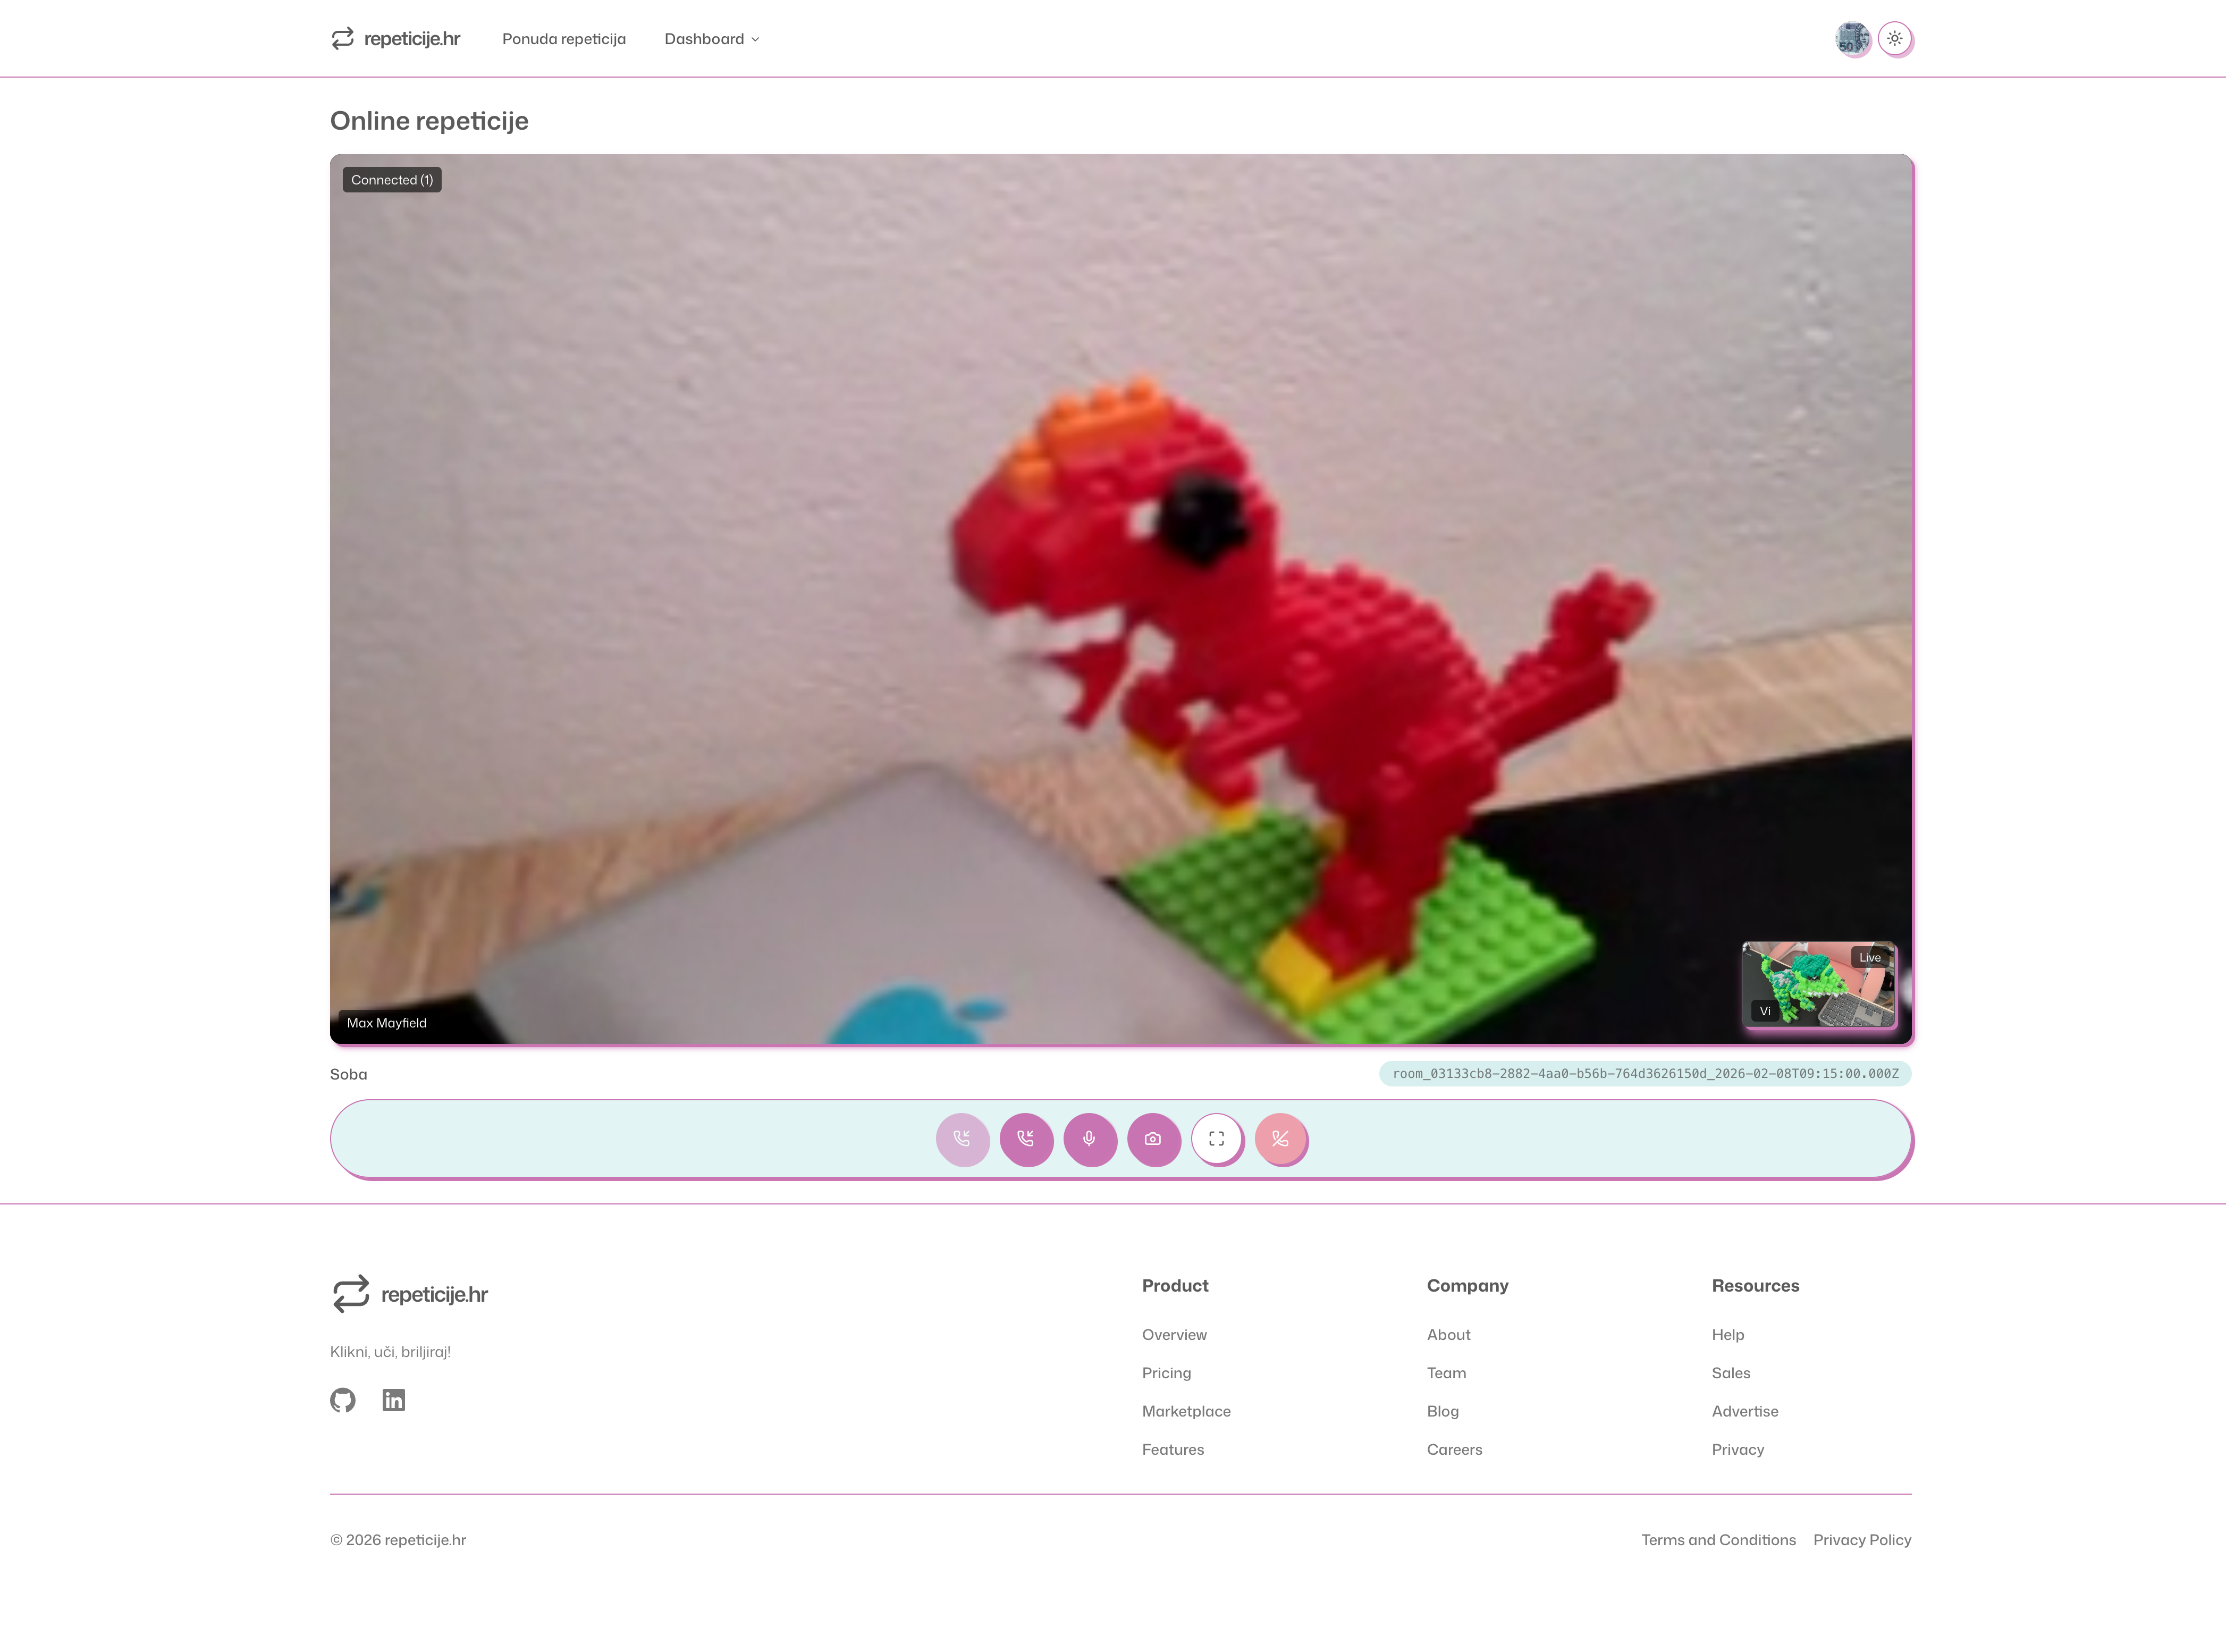
\includegraphics[width=\linewidth,clip]{assets/room-one-to-one-desktop.png}
    \caption{Soba za sastanke pri audio-video pozivu između dvaju sudionika (\textit{desktop}, macOS, Chrome)}\label{fig:call1To1Desktop}
  \end{minipage}
  \hfill
  \begin{minipage}{0.28\linewidth}
    \includegraphics[width=\linewidth,clip]{assets/room-one-to-one-mobile.jpeg}
    \caption{Soba za sastanke pri audio-video pozivu između dvaju sudionika (\textit{mobile}, Android, Chrome)}\label{fig:call1to1Mobile}
  \end{minipage}
\end{figure}

Na slikama~\ref{fig:callGroupDesktop} {--}~\ref{fig:callGroupMobile2} prikazana
je soba za sastanke pri audio-video pozivu između više sudionika (jedan tutor i
dva studenta), što ilustrira funkcionalnost grupnih \textit{online} repeticija
kroz različite preglednike, operativne sustave, uređaje i mrežne uvjete.

\begin{figure}[H]
  \centering
  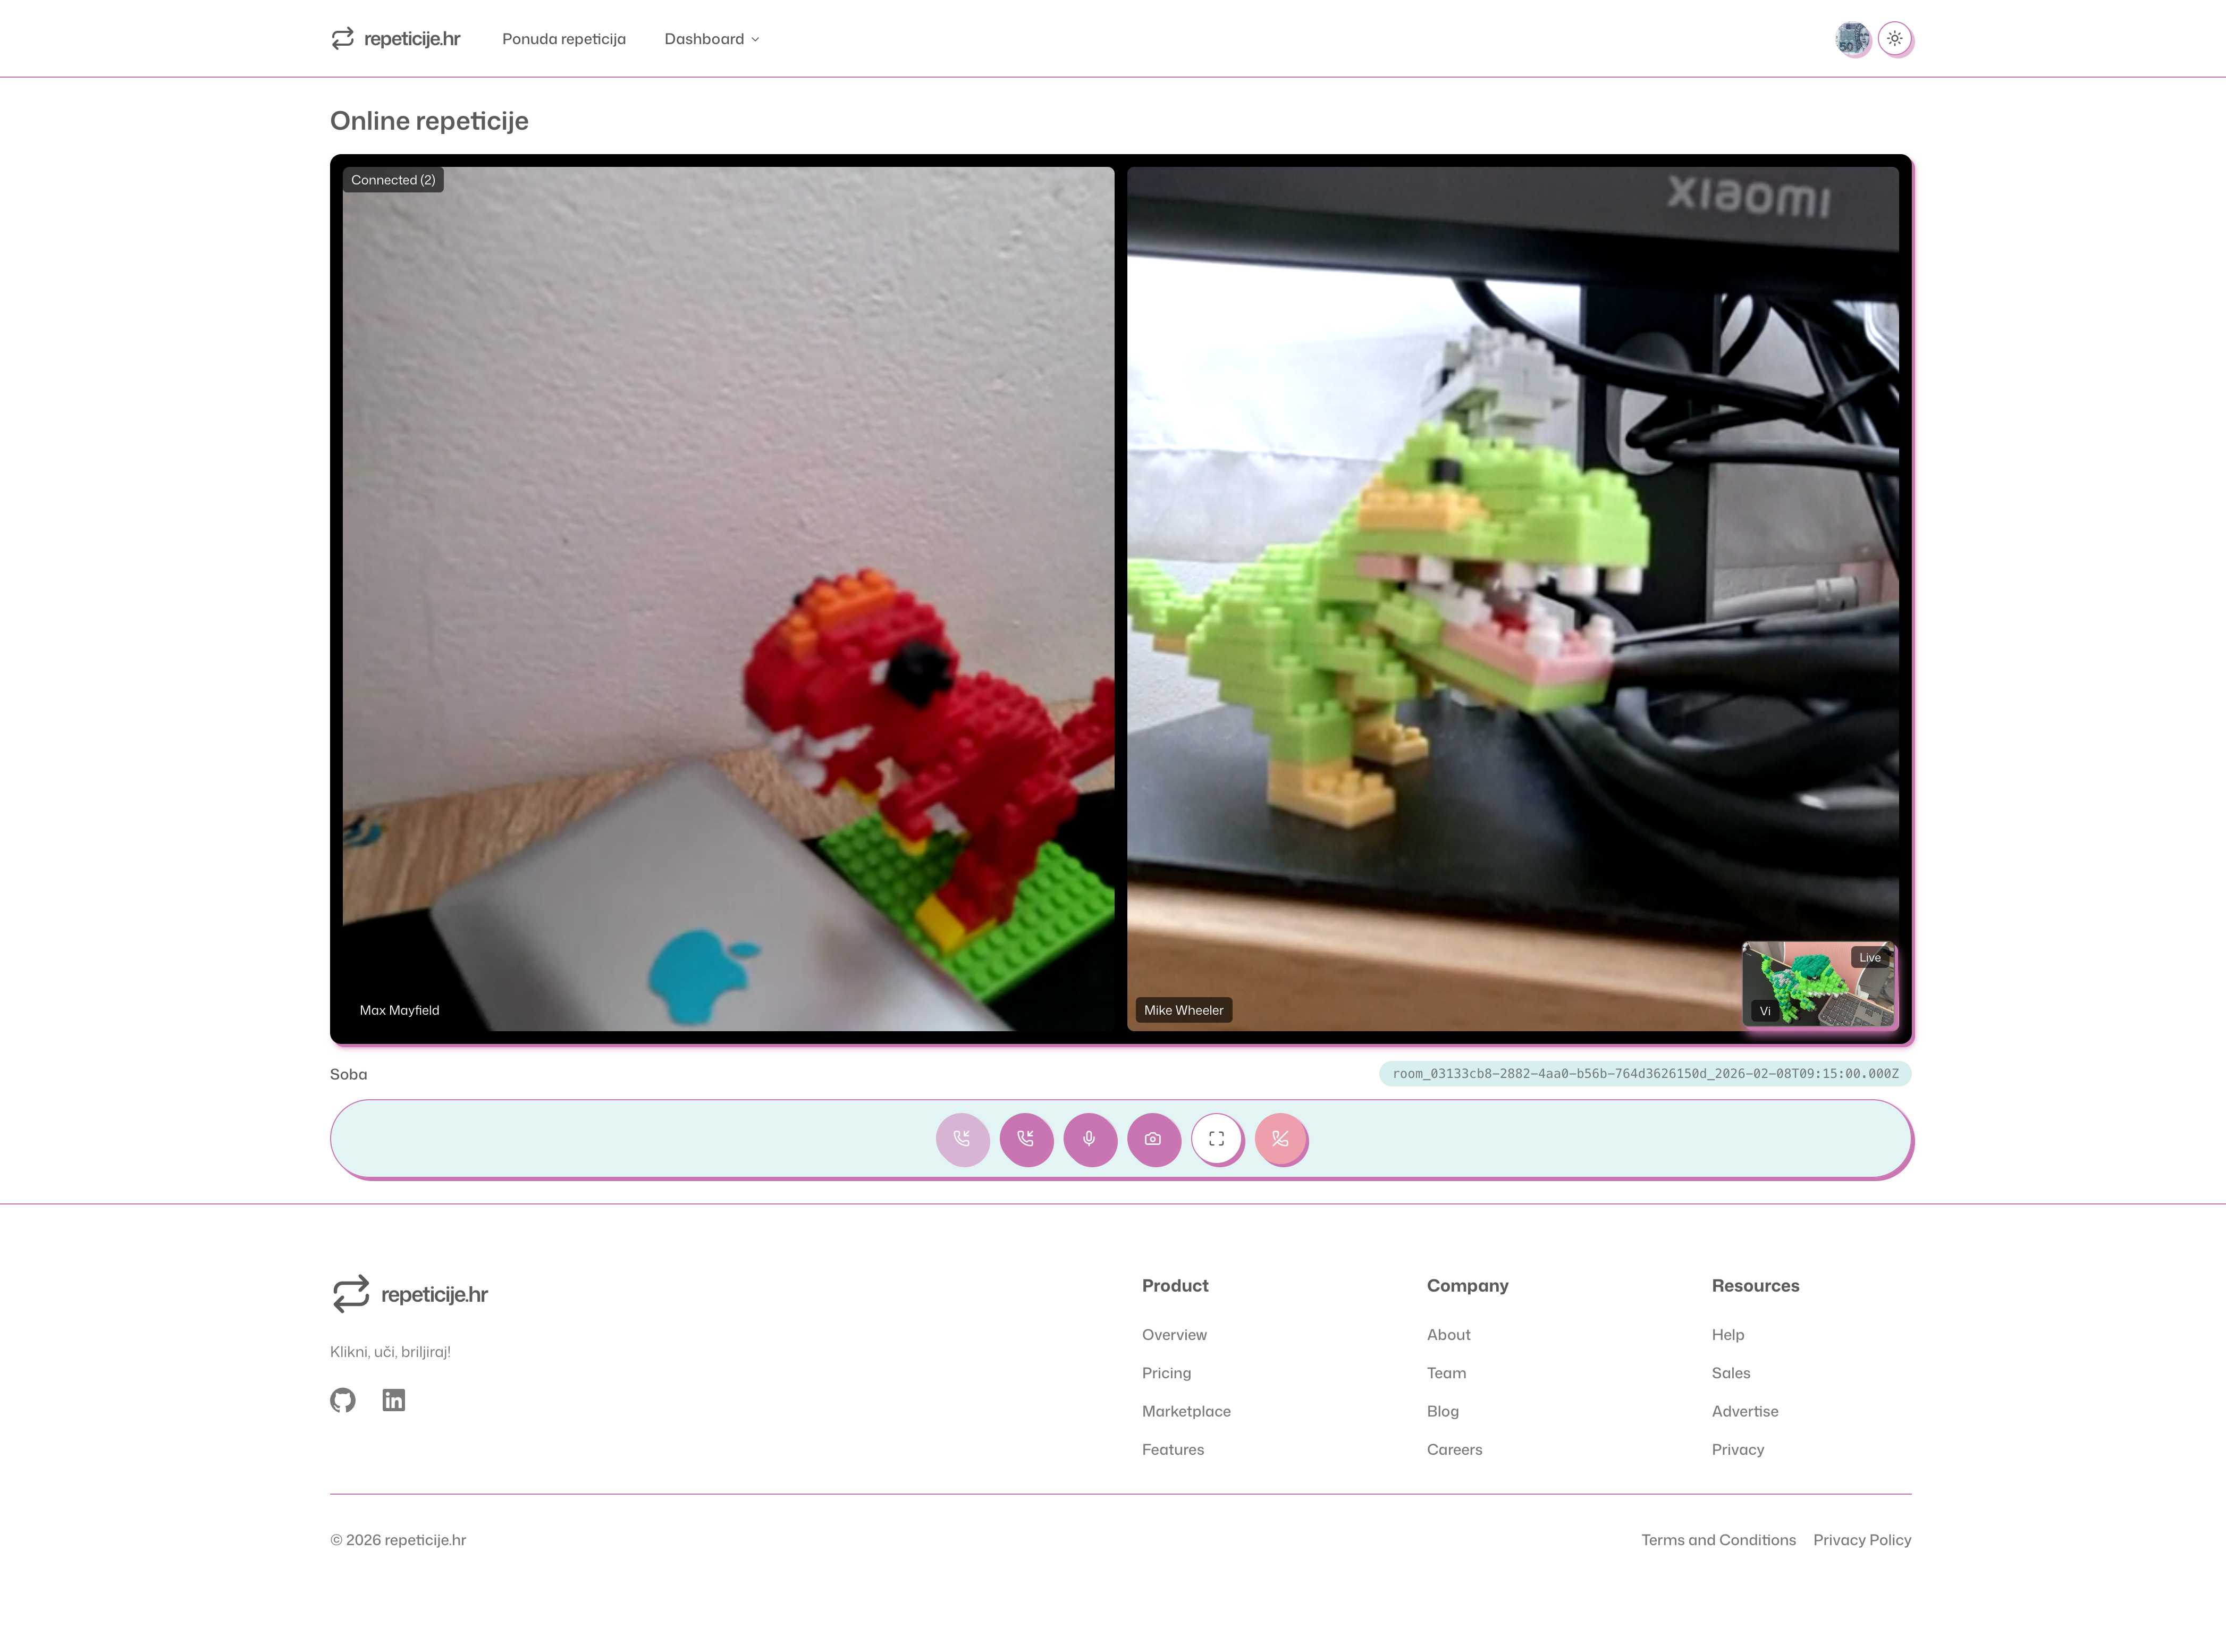
\includegraphics[width=0.9\linewidth,clip]{assets/room-group-desktop.png}
  \caption{Soba za sastanke pri audio-video pozivu između više sudionika (\textit{desktop}, macOS, Chrome)}\label{fig:callGroupDesktop}

  \vspace{0.5cm}

  \begin{minipage}{0.3\linewidth}
    \centering
    \includegraphics[width=\linewidth,clip]{assets/room-group-mobile-1.jpeg}
    \caption{Soba za sastanke pri audio-video pozivu između više sudionika (\textit{mobile}, Android, Chrome)}\label{fig:callGroupMobile1}
  \end{minipage}
  \hspace{1cm}
  \begin{minipage}{0.3\linewidth}
    \centering
    \includegraphics[width=\linewidth,clip]{assets/room-group-mobile-2.jpeg}
    \caption{Soba za sastanke pri audio-video pozivu između više sudionika (\textit{mobile}, Android, Samsung Internet)}\label{fig:callGroupMobile2}
  \end{minipage}
\end{figure}
